\chapter{Problem Analysis}
\label{cha:analysis}

There are a number of possible use cases in our problem domain. To demonstrate these cases we assume
we have a number of nodes and datasets respectively, but they are not necessarily on the same nodes.
In the following paragraphs we explain possible combinations of operations, nodes and datasets.

\section{Operation}
In every scenario we want to run an operation which could be linear or non-linear.

\subsection{Linear Operation}
Being linear means that the operation
could be broken into its components and then run in parallel or series. Here is algebic notation
of a linear operation which acts on two datasets:

\[ Operation(A + B) = Operation(A) + Operation(B) \]

Being linear or non-linear only matters when we have to operate on more that one dataset.

\subsection{Non-linear Operation}
In contrast to linear there is non-linear operation. This means that this kind of operation has dependant parts and
those parts could not run in parallel:

\[ Operation(A + B) \neq Operation(A) + Operation(B) \]

\section{Datasets}
For each operation we need one or more datasets which my be available on the same node that wants to run the operation
initially or could reside on other nodes. 

\subsection{Input}
Input files are normally not mission critical and could be reproduced.

\subsection{Output}
Operations create output datasets which normally are small in size, threfore we ignore the transfer cost of operation
results in our work.

\subsection{Data Locating}
We consider three different approaches toward preparing required data for operations.
\subsubsection{Conventional Approach}
in this approach we put the required data on a network file system and all
application instances will access it there. We will utilize an NFS mounted file system.
\subsubsection{Centralized Approach}
in this approach we will have a central instance which will orchestrate operation
delegation and operation output forwarding to other nodes.
\subsubsection{Decentralized Approach}
in this approach we will eliminate the orchestrator node and the network of
application instances should collaborate in a decentralized fashion to keep track of data and control flow for each
task.

For every approach we will run performance tests and we will compare the results.

\subsubsection{Method}
We will discuss scenarios in chapter\ref{cha:scenarios}. For each scenario we will analyze the possible combinations 
of data and operations and we will discuss how to 
deliver the input data and where to store output data. We will discuss workflow management in chapter 
\ref{cha:workflow} and data transfer in chapter\ref{cha:data}.


% TODO: I might need to introduce "Decision Tree"
\section{Decision Making}
The main decision that we need to make at every scenario is whether we should transfer the required data or we
need to delegate the operation to an instance on a node which already has the data. To make a decision we need to
answer a number of questions. First we need to know the location of the data:

\begin{enumerate}
\item Is the data available locally?
\item If not, is the data available on another node? -- Here only the physical location of data matters not the instance
controlling it.
\end{enumerate}

% TODO: Introduce "Decision Metrics"

%In case the mentioned data is available on another nodes we have to answer these questions:
%\begin{enumerate}
%\item What is the cost of data transfer? -- We have to invent an algorithm for this calculation
%\item If data is available on more than one remote node, which one has the minimum transfer cost? -- We might
%introduce multiple strategies and use some heuristics for this selection, simplest form would be random selection,
%another could be asking for an availability metric from the instance and mix it with local calculated availability 
%metric to get a final cost value.
% TODO: We can use "Heartbeat" concept as one of availability metrics
%\item In case it is expensive to transfer the data, can we delegate the operation to an instance on the other node?
%\end{enumerate}



\section{Concrete Scenarios}
We begin with a simple scenario and we gradually add details to it and build new scenarios.

\subsection{Scenario 1}
In this scenario we have a linear operation, e.g. \(Op^A\) on \(Node^A\) which
requires one single dataset such as \( Dataset^1 \) which is available on one of the other peers.

\subsubsection{Conditions} \( Dataset^1 \) is not available on \( Node^A \) and the operation is linear.
\subsubsection{Consequences} With these conditions we either should transfer \( Dataset^1 \)
to local node or in case of availability delegate \(Op^A\) to the node which already has \( Dataset^1 \).

\subsection{Scenario 1 (UC1)}
We have a distributed network of collaborating servers, where in this case, we consider two computers. 
Each server has its own storage and maintains a number of datasets on it. These servers collaborate 
together to accomplish issued commands. User in this case wants to perform one operation on a dataset
that resides only on one of the servers. There are two main assumptions here:
\begin{enumerate}
\item \textbf{The user has neither a prior knowledge where the data is stored}
\item \textbf{Nor of how many servers are present on the network}
\end{enumerate}

The user connects to one of the servers, which we call a client. This server is assumed to be part 
of the network, though it may not have any local data stores on it. The user issues, interactively
(or non-interactively) a command on a set of data providing some kind of identification. This command
is broadcast by the client to all servers in the network. All servers receive this command and check
whether they have the data locally. The server which has the data performs the operation and the others
ignore it. The result of the operation in this case, remains on the same server which the original 
dataset was on. 

\begin{itemize}
\item Note: it is assumed that at any instance of time, only one server acts as a client.
\end{itemize}

Moreover we assume the user has already queried the available data in the entire network by 
issuing something like “list datasets” which outputs dataset names and ids.

The following table shows two servers, each has one dataset. The user is connected to S2.\\

\begin{tabular}{ l c r }
\em{Server ID} & \em{ Dataset ID} & \em{ Client} \\
S1 & DS1 & No \\
S2 & DS2 & Yes \\
\end{tabular}\\

Let us assume the data sets are \(10^6\) random numbers.
Let us assume the operation is to transform the real random numbers to a set of [0 or 1 ] depending on whether the number is even or odd. 
This operation is assumed here to be a user defined method that operates on the data set.

\begin{itemize}
\item Note: A dataset can be for example defined as an object that has an id, and a one dimensional array (python list).
\end{itemize}

The user issues the command like this from a python shell: 

\begin{itemize}
\item real2bin(DS1) will result in -> Broadcast(real2bin(DS1))
\item Note: it is assumed that all functions are already defined on all servers, since they execute the same environment.
\end{itemize}

The client broadcasts this function to all servers. Each server will check if the data set with this id exists, if so will run the command. 

This means that each server, especially the client, has to “know about all data sets existing in all servers.
It does not need to have the actual data, but needs to know about it. So that when the user issues the command
above, he/she does not get a “data structure not existent” error from the client, just because the data is not
there. Hence we need some interface, or some wrapper function that checks the argument for the data type, or to 
create some proxy interface from all data to all nodes. 

\section{Assessing Suggested Approaches}
To be able to assess the performance of each given solution to the mentioned scenarios we made a demo application
called \textbf{Konsensus}. The code is available on Github. %TODO add ref here

\subsection{Testing Problems}
Writing tests for a distributed application is not as easy as writing unit-tests for a normal application. 
Our demo application acts as a server and client at the same time. Moreover we want to launch multiple 
network peers running on one or more machines. Testing scenarios on this network is not possible with
normal mocking approaches, because we need to test the behavior of our solution in a network of collaborating
peers which are not external, rather the core services of the application.

To overcome testing issues we have to launch the desired number of peers separately and then run our tests 
over them. To make this operation faster we changed the application to make it possible to launch any number
of instances on one machine and we automated this process using a number of scripts. %TODO more details

\subsubsection{Mixing Signals in Greenlets}
We use python Greenlets instead of threads. This means that our demo application runs on only one thread. 
This causes a problem when launching multiple apps all together with one script and inside one thread, that
causes the signals for events spread among all greenlets and make trouble. To avoid this we have to run
each server in a separate processes. Running them inside threads won't help as well because the blinker python
library is thread-safe so it moves signals between threads as well as Greenlets.

\subsection{Scenario 2 (UC2)}
This is similar to scenario one, except that the operation requires two datasets to be done. We have a network of peers collaborating
to finish some linear and non-linear tasks. In this scenario we need at least three peers involved. We assume the first peer has no
data of our interest therefore it should cooperate with others to accomplish the request. Our operation in this case requires two 
different datasets which are not available on the first peer and we should access them on other peers. The main points the same:

\begin{enumerate}
\item \textbf{The user has neither a prior knowledge where the datasets are stored}
\item \textbf{Nor of how many servers are present on the network}
\item \textbf{The operation is linear}
\end{enumerate}

We assume the data distribution is like the following table:

\begin{tabular}{ l c r }
\em{Server ID} & \em{ Dataset ID} & \em{ Client} \\
S0 & --- & Yes \\
S1 & DS1 & No \\
S2 & DS2 & No \\
\end{tabular}\\

\subsubsection{Possible Approach}
In order to calculate the result we might take a number of approachers, we start with a combination of \textbf{divide and conquer} and
\textbf{produce-consume-collect} methods.

The S0, in this case, is the peer who receives the command and initiates the request. The two other peers, S1 and S2 respectively, have the required
datasets. The initiator will find the corresponding datasets and will dispatch commands to run each part on each peer and then will collect
the resulting datasets. This will be a blocking operation, we will wait until the other peers finish their parts and return the result
to us. If the output is a number it will be returned to the user, if it is a dataset it will be stored based on defined storage mechanism, 
currently we use random storage. The peer will break the operation into smaller operations each one calculating result for one of datasets, 
this \textbf{sub-operations} will be executed like \textbf{scenario 1} and the result will be collected by initiator peer.

We assume that in this case we have two arrays, each consisting of \(10^6\) random numbers. We have to first transform these datasets into
a set of [0 or 1] based on the number being even or odd (use case 1) and then we make a third dataset which contains the sum of every two
corresponding numbers in range of [0 to 2].


\begin{itemize}
\item Note: in this case each pear should be able to run the requested linear operation on one or more datasets.
\end{itemize}

The notation of above mentioned approach will be like this:

\[ Operation(A + B) = Operation(A) + Operation(B) \]

In order to run this operation in a collective way, we need to think of the type of service calls in our system, whether they are blocking or
non-blocking. Since often the operations in HPC environments are time consuming and long-running, we consider the non-blocking approach. In
this way the user will provide a dataset name for storing the result. The operation will be \textbf{submitted} to the collaborative network.
Later on user is able to query for the result using the key that she had provided at the time of submission. This allows us to design our system
in a more decentralized way, where each peer can inform others (neighbors) about a request in a \textbf{publish-subscribe} manner, where the peer
will publish a request and finish the operation. Later on the peer who has the dataset will \textbf{react} to the published request and will take
further actions, all the other peers who do not have the requirements (the dataset for now) will ignore it, however they can store the details of 
running operations for next steps, when we will come to more complex workflow.

To show more detailed version of this operation we demonstrate the steps for it:

\begin{enumerate}
\item User issues the command to S0, providing DS1, DS2 \st{and a unique name for the result}
\item System will check whether the operation is linear
\item Then it will break the command into sub-commands, each for one of datasets
\item System will generate unique ids for each sub-command
\item System will then submit the sub-commands along with dataset name and the unique id for the result dataset
to \textbf{itself}, which will cause a situation like scenario 1
\item System will next have to collect the results in a non-blocking manner which we will discuss shortly.
\end{enumerate}

\begin{itemize}
\item With the use of operation ids we eliminate the need to get a result dataset name from user but we still can accpte \textbf{tags} from users.
\end{itemize}

\begin{itemize}
\item We assume every operation involving more than one dataset is made of other operations which are already defined in the system.
\end{itemize}

There is an important issue here, we create sub-operations for each operation and we run them in a non-blocking manner, this will
cause it almost impossible to return the result of operation to the user in one run. One might think that we can block and query
until the result of sub-operations are ready, but this is something that we want to avoid. Therefore to solve this issue in a 
distributed manner, we introduce an operation id for each user request. We inform all the peers via sending messages (signals) about
the new operation and it's id and sub-commands. Each peer will update this operation internally based on further received messages.
We also return the operation id to the user instead of any results. Then user will query for the result of operation, providing the 
operation id. We change the above steps like this:

\begin{enumerate}
\item User issues the command to S0, providing DS1, DS2 and a unique name for the result
\item \textbf{System will generate a unique id for the operation and will store it along with the parameters}
\item System will check whether the operation is linear
\item Then it will break the command into sub-commands, each for one of datasets
\item System will generate unique ids for each sub-command
\item \textbf{System will notify other peers about the incoming operation with related parameters}
\item System will then submit the sub-commands along with dataset name and the unique id for the result dataset
to \textbf{itself}, which will cause a situation like scenario 1
\item System will next have to collect the results in a non-blocking manner which we will discuss shortly.
\item System will return the operation id to the user
\end{enumerate}

In the other hand the other peers which are the same basically, will react to the new operation signal:

\begin{enumerate}
\item Receive operation update message
\item Make a local lookup if the operation should be added or updated
\item Add or update the operation in the local storage
\end{enumerate}

Having the operation id and local updating storage for operations we now need to find a way to collect the results.
First of all we need to decide which peer will collect the results. We take the most straigh forward for now, the 
initiator peer, which has the knowledge of existing datasets in the network along with their sizes, will pick the 
peer which contains the largest dataset as the collector peer. We explicitly decide about the collector node in the
beginning either by size or randomly amount the data container peers.

It is worthy to mention that the collector peer will then store the result based on the configured storage mechanism 
which is random storage for now, not necessarily storing on the same node.

Now we have enough information in each peer to collect, process and store the results. The peers (including the collector)
 will react to operation methods like this:

\begin{enumerate}
\item Receive operation update message
\item Make a local lookup if the operation should be added or updated
\item Add or update the operation in the local storage
\item Am I the collector? If yes do the followings:
\begin{itemize}
\item check if the sub-operations are done
\item If the sub-operations are done, collect their results
\item Process the results
\item Based on the storage mechanism store the result
\item Update the operation with the result dataset id
\item Change status of operation to "done" (we need a proper state-machine here)
\item Inform other peers about the update
\end{itemize}
\end{enumerate}

Now if user makes a query giving the operation id this would be the result:

\begin{enumerate}
\item Check operation storage
\item If the operation is marked done, return the dataset id
\item If it is not done, return the status.
\end{enumerate}

\section{Operation Implementation}
About implementation of operation decorator (aspect?)

\section{Observed Errors}
While testing scenario 2 we observed a common error. We this scenario with three different peers as the following table:

\begin{tabular}{ l c r }
\em{Server ID} & \em{ Dataset ID} & \em{ Client} \\
S0 & --- & Yes \\
S1 & DS1 & No \\
S2 & DS2 & No \\
\end{tabular}\\

We also used \textbf{Random Dataset Storage} mechanism, simply to store resulting dataset of one operation on one of the network
peers. The problem is when two peers decide to store the result of one operation on each other a blocking condition happens. Our
approach was opening a temporary port and inform the other peer to fetch the data. Meanwhile this is exactly happening on the other
peer, therefore both block.

\subsection{Solution}
To solve the blocking peers problem we used the already running main application API instead of opening temporary PULL/PUSH zeromq 
sockets. This change is working fine and the peers exchanging datasets with no problem.

\section{Show Cases}

In this chapter we will go through a set of experiments to showcase the result of taking different approaches toward file transfer techniques. Meanwhile we will try a number of data distribution methods to see how they fit into our scenarios.

\section{Distributed Hash Tables}
Distributed Hash Tables (DHT) known best for their application to build torrent tracking software, let us to have a key/value store and distributed it in a decentralized way amount a network of peers.

MORE INFO HERE ON DHT, KAMEDLIA PAPER and IMPLEMENTATIONS

In our case to keep track of the available data on the network of collaborating peers, we can use a DHT table. Every time an instance wants to find a dataset it should query the network of peers using one of the existing wrappers and implementations.

\section{Test Results}
Our tests show that even though DHT is fault-tolerant and reliable for file distribution, it is not adequate for our realtime requirement to find our required data. In one test we ran two peers, one on an Internet host and another one on local host. Here are the client and server codes:

\begin{python}
from twisted.application import service, internet
from twisted.python.log import ILogObserver

import sys, os
sys.path.append(os.path.dirname(__file__))
from kademlia.network import Server
from kademlia import log

application = service.Application("kademlia")
application.setComponent(ILogObserver, 
	log.FileLogObserver(sys.stdout, log.INFO).emit)

if os.path.isfile('cache.pickle'):
    kserver = Server.loadState('cache.pickle')
else:
    kserver = Server()
    kserver.bootstrap([("178.62.215.131", 8468)])
kserver.saveStateRegularly('cache.pickle', 10)

server = internet.UDPServer(8468, kserver.protocol)
server.setServiceParent(application)


# Exposing Kademlia get/set API
from txzmq import ZmqEndpoint, ZmqFactory, ZmqREPConnection,
 ZmqREQConnection

zf = ZmqFactory()
e = ZmqEndpoint("bind", "tcp://127.0.0.1:40001")

s = ZmqREPConnection(zf, e)

def getDone(result, msgId, s):
    print "Key result:", result
    s.reply(msgId, str(result))

def doGetSet(msgId, *args):
    print("Inside doPrint")
    print msgId, args

    if args[0] == "set:":
        kserver.set(args[1], args[2])
        s.reply(msgId, 'OK')
    elif args[0] == "get:":
        print args[1]
        kserver.get(args[1]).addCallback(getDone, msgId, s)
    else:
        s.reply(msgId, "Err")

s.gotMessage = doGetSet
\end{python}

In the above example we have used \textit{twisted} networking library\cite{TwistedMatrix} and one python implementation\cite{KademliaImpl} of \textit{Kademlia} DHT algorithm\cite{KademliaPaper}. This will start a p2p network and will try to bootstrap it with another peer on the give IP address. Thereafter it will open another endpoint to expose a simple \textit{get/set} method for the rest of application for communicating with the network.

HERE DESCRIBE ABOUT DHT IMPLEMENTATION AND TWISTED NETWORKING LIBRARY. ***MOST IMPORTANT*** ABOUT REPLICATION OF DATA, IS THERE ANY REPLICATION? WHAT IF A NETWORK NODE FAILS? ***RCP OVER UDP AND WORK THROUGH FIREWALLS***

The next part is a few lines of code to communicate with this network:

\begin{python}
#
# Request-reply client in Python
# Connects REQ socket to tcp://localhost:5559
# Sends "Hello" to server, expects "World" back
#
import zmq

# Prepare our context and sockets
context = zmq.Context()
socket = context.socket(zmq.REQ)
socket.connect("tcp://localhost:40001")

# Set request
socket.send(b"set:", zmq.SNDMORE)
socket.send(b"the key", zmq.SNDMORE)
socket.send(b"the value")
print socket.recv()

# Get request
socket.send(b"get:", zmq.SNDMORE)
socket.send(b"the key")
print socket.recv()

# Invalid get
socket.send(b"get:", zmq.SNDMORE)
socket.send(b"not existing")
print socket.recv()
\end{python}

This simple client will try to connect to the previously opened port and send get/set messages.

\subsection{The Problem}
Configuring this p2p network is a little tricky. The network should work correctly even if nodes enter and leave the network. During our tests in development environment we observed some problems with initializing the network, but while the network was initialized leaving and entering the network had no effect on the results.

\subsubsection{Reliability}
Having the number of nodes increased up to 3 the reliability shows up again. When we set a value for a key in one node we can not guarantee that getting the value for that key on other nodes will return the updated one. With a number of tests I can confirm that two nodes which are bootstrapped with the same third node does not provide the accurate result every time and it is not clear for me why this happens. See figure~\ref{fig:threepeers} on page ~\pageref{fig:threepeers}.

After running more tests, we figured out that the possible source of the above mentioned problems was the confusion in using \textit{binary} and \textit{string} in python, so it was an error in our side.

\begin{figure}
\centering
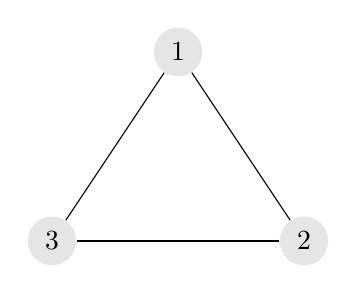
\begin{tikzpicture}
  [scale=.8,auto=left,every node/.style={circle,fill=gray!20}]
  \node (n1) at (5,5) {1};
  \node (n2) at (7,2)  {2};
  \node (n3) at (3,2)  {3};

  \foreach \from/\to in {n1/n2,n1/n3,n2/n3}
    \draw (\from) -- (\to);
\end{tikzpicture}
\caption{A network of three peers}
\label{fig:threepeers}
\end{figure}


\subsubsection{Firewall Problems}
In a test having one process running on a server in Internet and outside of the local network and having two different processes running on one laptop but on different ports it is observed that the changes (sets) in the Internet does not replicate to the local processes but the changes from local processes are being replicated to the other process.

\subsection{conclusion}
Having a network between local and Internet processes in the above mentioned method is not reliable. Repeating the tests with only local processes which are bootstrapping to one of them and running the setter/getter methods showed that even in this scenario it is not reliable and one can not guarantee that the desired value will be returned.


\section{Network Programming}
To showcase our desired approach and trying different ones we have used a number of network programming frameworks for python programming language. The main library that we use is called ØMQ or ZeroMQ~\cite{ZeroMQ}. ZeroMQ is an asynchronous messaging library written in C with bindings for many languages including python. This library helps us to easily scale and use different programming paradigms such as publish-subscribe, request-replay and push-pull.

\section{Publish-Subsribe Method}
Because of reliability issues we fall back to use a simpler approach using ZeroMQ. In this stage our aim is to distribute the information about available datasets at each node. To achieve this we let our demo application launch a number of communicators and publish information about it's data. Other nodes in our network have to subscribes on other nodes, hopefully ZeroMQ allows us to subscribe to multiple publishers, therefore each node can subscribe to other nodes. Nodes frequently get \textbf{news} from other nodes, for example availability of certain datasets on a node, then it can use publish-subscribe to get extra information on that particular subject.

\subsection{Architecture}
For demonstration purposes we create a python console application using Gevent\footnote{\url{http://www.gevent.org/}}, zeromq\footnote{\url{http://zeromq.org/}} and zerorpc\footnote{\url{http://zerorpc.dotcloud.com/}} to be able to service multiple requests in a non-blocking fashion.

\subsubsection{Application Initialization}
First of all each application instance establish its own zeromq publisher socket. Then it subscribes itself to all other nodes which are listed in config file. At this stage it should be configured manually.

\subsubsection{Gevent and non-blocking}
HERE WRITE ABOUT GEVENT.

\subsection{Exposing API}
Since this is going to be a network program we need to use a form of Remote Procedure Call (RPC) to communicate between nodes. Rather than implementing ourselves we used a library based on zeromq called \textit{zerorpc}. Using this library we now expose a set of APIs and let the nodes talk to each other based on this API. There are multiple solutions for exposing services which we do not discuss here.

\subsubsection{Data transfer using zerorpc}
WHICH DATA TYPES ARE WE ALLOWED TO TRANSFER USING ZERORPCS? IS IT ENOUGH FOR US?

\subsection{Application's State}
WE HAVE TO DECIDE ON A STATE MANAGER TO MAKE APPLICATION'S BEHAVIOR RELIABLE.

\subsection{Network Discovery}
At this stage there is no network discovery, because it is not our main problem. It can be done later as an improvement.

\subsection{Failure Recovery}
Again this is not of our interest. The point is there are existing solutions for these problems and we want to let our application to be able to demonstrate the main problem which would be deciding about data transfer routes and distributing the information about currently running operations.

\section{Use Case One Problems}
When we ask for an operation and we want to store the result somewhere on the network we have to think about the result name. 
We need a consistent way of naming datasets. If we ask users to provide resulting dataset names it will break soon, we need to 
let user to somehow give some \textbf{tags} but not the real names. We have to let the user know about the result name but also
let her to look for datasets by providing some tags.

The simplest problems that will happen if we store datasets with similar names is redundant work in the network. Peers will start 
to process and override the same dataset.

\subsection{Data Manipulation}
We will neet to let users to manipulate currently existing datasets, but very fast it comes to mind that not every dataset should be
writable, we will need to categorize and identify our datasets based on some criteria. These problems are not part of my thesis but
We mention it as part of problem analysis.



\section{Rough Ideas}

This chapter contains very raw ideas to address main requirements i.e.
distributed workflow management and intelligent data transfer.

\section{Intelligent Data Transfer: Use Case One}
By \textit{Intelligent Data Transfer} we mean an approach that
minimizes required data transfers between application\footnote{To be defined}
instances.

In the most basic use case\footnote{To be added later and 
referenced here} we run a script
\footnote{To be defined and added to
the terminology, terminology itself has to be defined}
which consists of two linear operations. Each operation consumes data
and generates data. A third operation needs both generated data two 
operate on and generate the third and final data.

The script is data driven. It means that it contains a number
of steps and for every step it needs appropriate data to run the
desired operations\footnote{To be defined}. We assume that
the script will run on \textit{Node 1} and required data 
\textit{DataSet1} and \textit{DataSet2} are 
located on \textit{Node 2}
and \textit{Node 3} respectively. Therefor \textit{Node 1} have
to initiate operations on the other machines.

\subsection{Identical Instances}
We assume that on each machine of the network the same instance of our program is running which 
is capable of all of our operations
including A, B and C. The only consideration is the availability of 
Datasets, they are not available on all machines.

A linear operation (not clear to my self how to write it):

\[ Operation(A, B) = Operation(A) + Operation(B) \]

\[ DataSet^A = Operation^A(DataSet^1) \]

\[ DataSet^B = Operation^B(DataSet^2) \]

\[ DataSet^C = Operation^C(DataSet^A, DataSet^B) \]

Assuming that operations A and B will run on the machines which
contain the required data, a number of questions arise here:
\begin{enumerate}
\item On which machine operations C should run? A, B or C?
\item On How to transfer the required data to that machine in an 
optimized way?
\end{enumerate}

\subsection{The Idea}
First of all we assume that we have the information about the Datasets
available on all of the machines i.e. in form of a distributed table
with entries containing the node address and Dataset id. Based on this
information the application can decide if it has the required data or
not. 

Based on this algorithm (to be defined) the initial application
delegates operations to the other nodes (instances of the same program),
where the data is available. Our distributed workflow manager (to be 
defined) will synchronize the information on these running operation and
will label the output data and will add it to the distributed data table.

After finishing operations A and B we will run operation C in either
of these nodes, because the required data is partially available on these
nodes. Then we have to transfer the rest of the data to one of these
nodes to run the operation C which needs both parts simultaneously.

\subparagraph{Using Prior Art}
At this point we can take advantage of existing Distributed File Systems
(DFS) to make the data available for operation C. We can then eliminate
the complexity of data transfer between these two nodes and delegate it
to existing distributed file systems. The main point is we don't rely on
DFS for all of our decision making part but we explicitly make the 
decision to run operation A and B on specific nodes and then for the 
last part we use a meta or universal disk concept to deliver the
remaining data for operation C.

\section{Sqmpy Integration}
We can use Sqmpy project as a monitoring tool for konsensus network.
 Providing one peer address it can query the rest of peers and connect or 
subscribe to their news channel. Having this we can always see which nodes are
offline and which ones are online. This also gives us a platform to extend
monitoring and control features to the web. Currently we have made all the 
required software platform to achieve this. On Sqmpy side using Flask microframework
and socket.io we can simply maintain realtime connections to the browsers and since
our web framework is written in python, with minimum cost we can integrate it
with konsensus.
